\documentclass{article}

\usepackage{graphicx}
\usepackage{tikz}
\usepackage{tikzsymbols}
\usetikzlibrary{calc,patterns,shapes.geometric}
\pagestyle{empty}
\usepackage[margin=0pt]{geometry}
\geometry{papersize={14in,12in}}

\def\centerarc[#1](#2)(#3:#4:#5){\draw[#1] ($(#2)+({#5*cos(#3)},{#5*sin(#3)})$) arc (#3:#4:#5);}

\begin{document}
	\begin{figure}
		\centering
		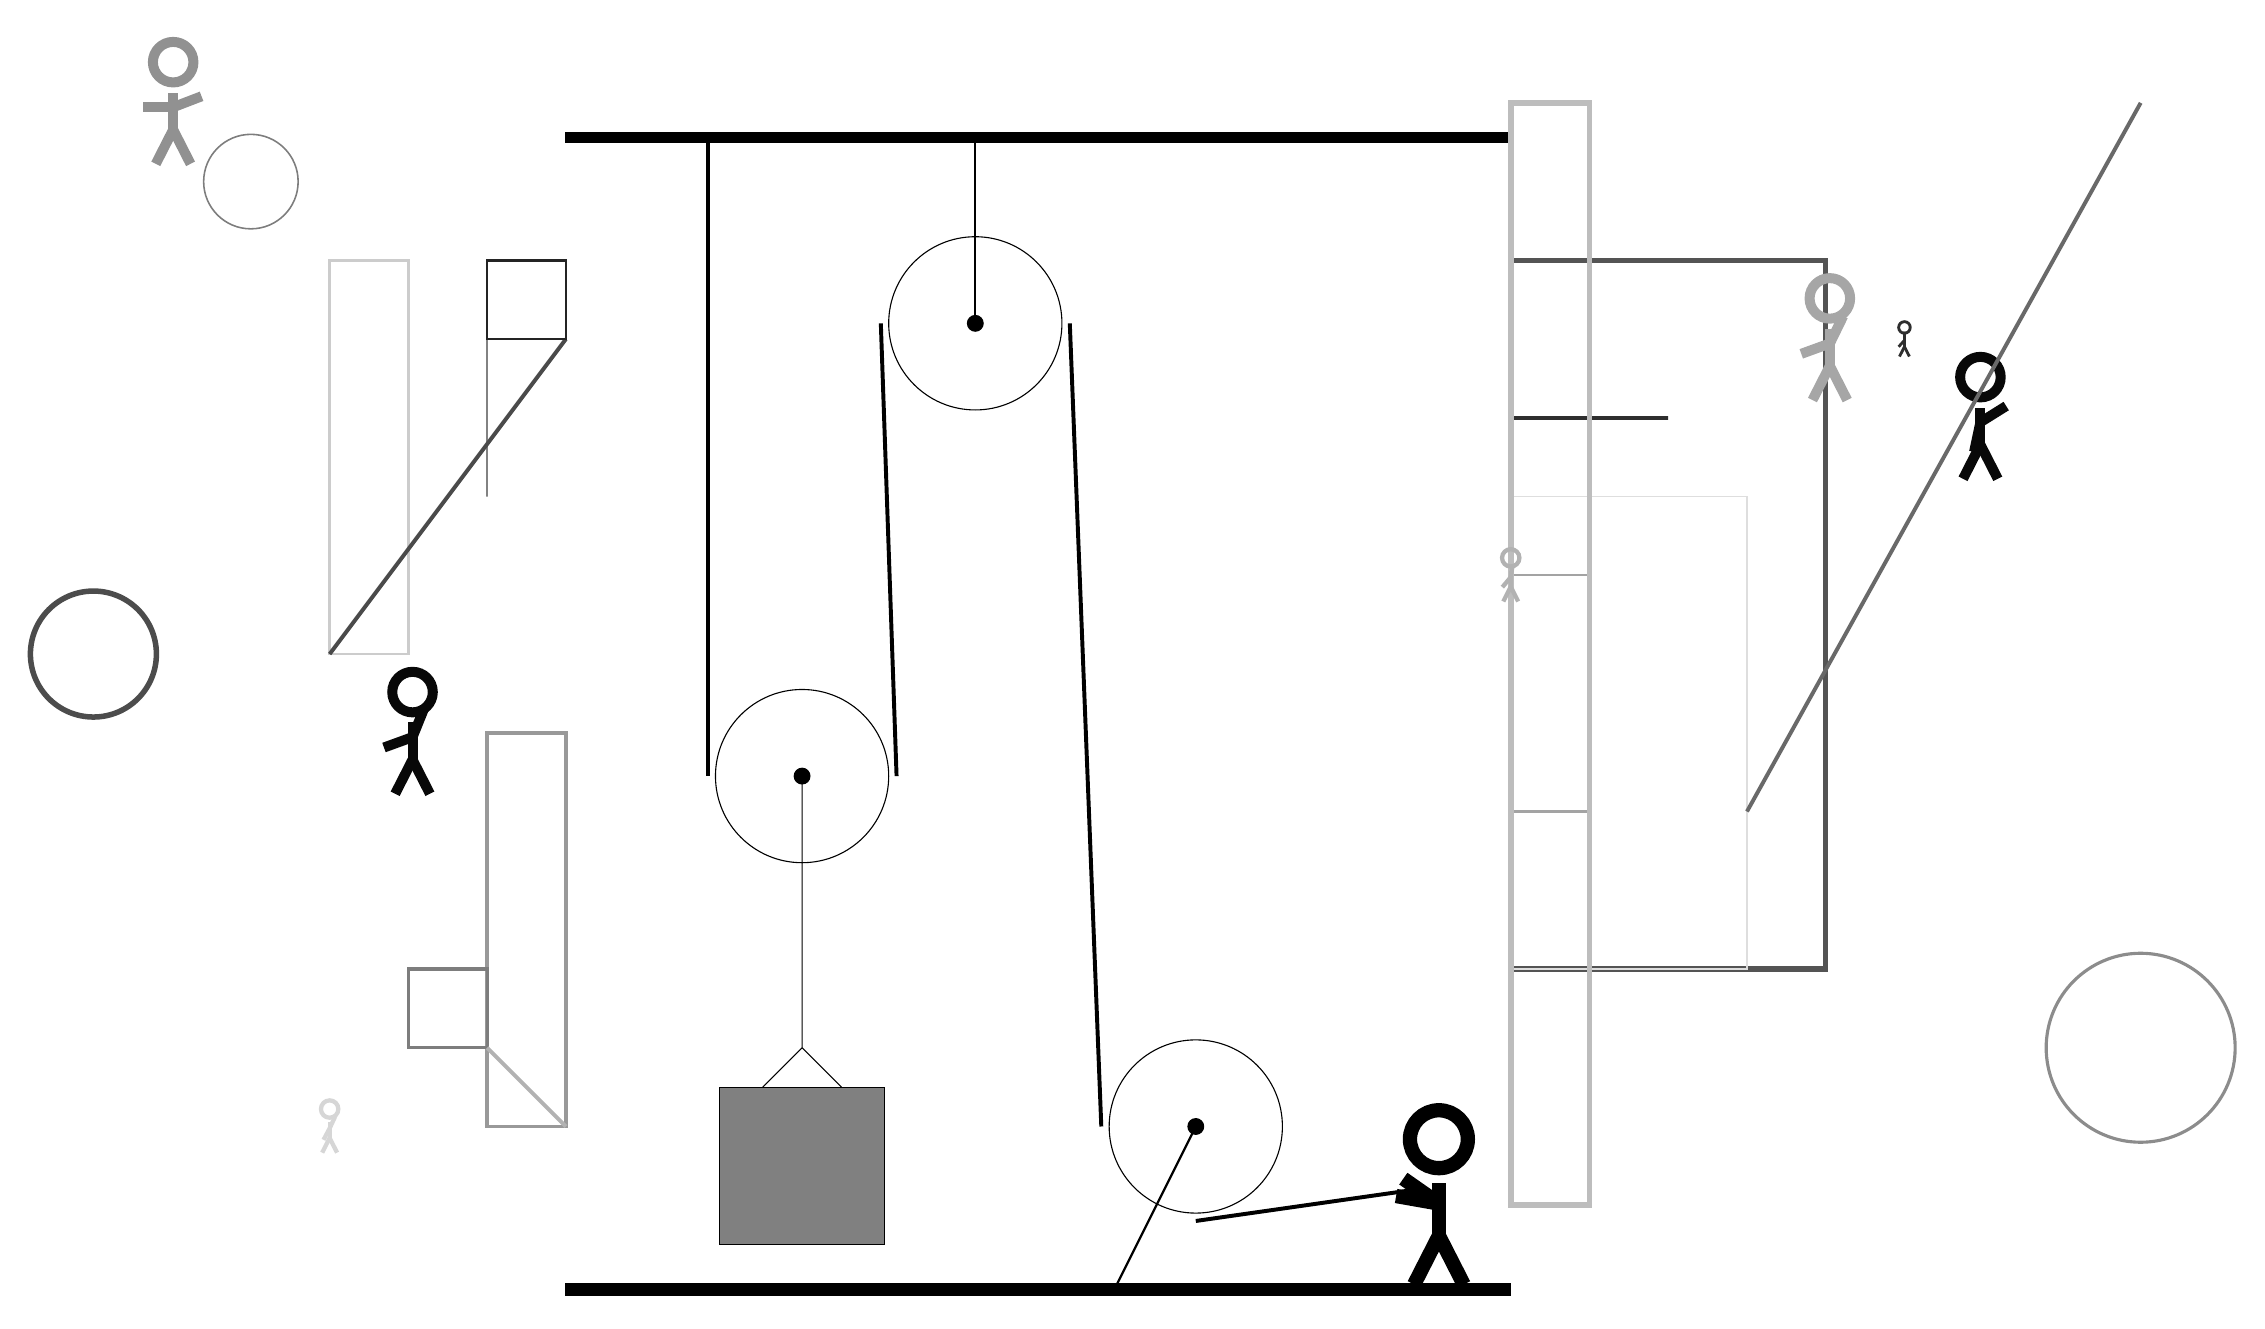
\begin{tikzpicture}
			%%%%% START %%%%%
			
			\draw[fill=black] (-2, 11.5) rectangle (10, 11.625);
			
			\draw (3.2, 9.2) circle (1.1);
			\draw[fill=black] (3.2, 9.2) circle (0.1);
			\draw[thick] (3.2, 9.2) -- (3.2, 11.5);
			
			\draw (6, -1) circle (1.1);
			\draw[fill=black] (6, -1) circle (0.1);
			\draw[thick] (6, -1) -- (5, -3);
			
			\draw (1, 3.45) circle (1.1);
			\draw[fill=black] (1, 3.45) circle (0.1);
			
			\node[line width=0.4mm, color=black!82] at (15, 9) {\Strichmaxerl[2][48][89]};
			
			\draw[line width=0.2mm, color=black!49] (-3, 7) rectangle (-3, 10);
			\node[line width=0.3mm, color=black!43] at (-7, 12) {\Strichmaxerl[7][0][21]};
			\node[line width=0.6mm, color=black!97] at (-4, 4) {\Strichmaxerl[7][20][68]};
			
			\draw[line width=0.3mm, color=black!20] (-4, 10) rectangle (-5, 5);
			
			\node[line width=0.5mm, color=black!97] at (16, 8) {\Strichmaxerl[7][78][32]};
			
			\draw[line width=0.5mm, color=black!40] (-2, -1) rectangle (-3, 4);
			
			\draw [line width=0.7mm, color=black!70](-8, 5) circle (0.8);
			\draw[line width=0.7mm, color=black!67] (10, 1) rectangle (14, 10);
			
			\draw[line width=0.2mm, color=black!13] (10, 1) rectangle (13, 7);
			
			\draw[line width=0.5mm, color=black!82] (10, 8) rectangle (12, 8);
			
			\draw[line width=0.5mm, color=black!71](-5, 5) -- (-2, 9);
			\draw [line width=0.2mm, color=black!51](-6, 11) circle (0.6);
			\node[line width=0.6mm, color=black!16] at (-5, -1) {\Strichmaxerl[3][62][65]};
			\draw[line width=0.5mm, color=black!59](13, 3) -- (18, 12);
			\draw[line width=0.3mm, color=black!36] (10, 3) rectangle (11, 6);
			\draw[line width=0.7mm, color=black!26] (11, -2) rectangle (10, 12);
			\node[line width=0.4mm, color=black!35] at (14, 9) {\Strichmaxerl[7][20][64]};
			\draw[line width=0.3mm, color=black!86] (-3, 10) rectangle (-2, 9);
			\draw[line width=0.4mm, color=black!51] (-4, 1) rectangle (-3, 0);
			\draw[line width=0.5mm, color=black!30](-2, -1) -- (-3, 0);
			\node[line width=0.3mm, color=black!30] at (10, 6) {\Strichmaxerl[3][50][81]};
			\draw [line width=0.4mm, color=black!45](18, 0) circle (1.2);
			
			\draw (1, 3.45) -- (1, 0.0) -- (0.5, -0.5);
			\draw (1, 0.0) -- (1.5, -0.5);
			\draw[fill=black!50] (-0.05, -0.5) rectangle (2.05, -2.5);
			
			\draw[line width=0.5mm] (-0.2, 11.5) -- (-0.2, 3.45);
			\centerarc[line width=0.5mm](1, 3.45)(180:360:1.2000000000000002);
			\draw[line width=0.5mm](2.2, 3.45) -- (2.0, 9.2);
			\centerarc[line width=0.5mm](3.2, 9.2)(0:180:1.2000000000000002);
			\draw[line width=0.5mm](4.4, 9.2) -- (4.8, -1);
			\centerarc[line width=0.5mm](6, -1)(180:270:1.2000000000000002);
			\draw[line width=0.5mm](6, -2.2) -- (8.8, -1.8);
			
			\node at (9, -1.9) {\Strichmaxerl[10][-35][170]};
			
			\draw[fill=black] (-2, -3) rectangle (10, -3.15);
			
			%%%%% END %%%%%
		\end{tikzpicture}
	\end{figure}	
\end{document}